% Fixture "names": a student report full of personal data, for pseudonymization (spec §10, §12.1).
% Deliberately leaves pdfTeX's PTEX keys on and exercises every location of §10.3:
% - OT1 encoding, so umlauts are a base letter plus a separate accent glyph (combining-accent case)
% - names with possessives (English and German), upper case, a name hyphenated across lines,
%   a name with an ffi ligature, an e-mail address and a student ID
% - hyperref Info (Author, Title, Subject, Keywords), XMP metadata (hyperxmp), outlines with names,
%   link annotations (mailto, citation), named destinations with a name (cite.mueller2020),
%   an embedded file, a form field, OpenAction JavaScript, and an included PDF page (PTEX.FileName,
%   PTEX.InfoDict) whose text contains a name.
\documentclass[11pt]{article}
\usepackage[utf8]{inputenc}
\usepackage{graphicx}
\usepackage{embedfile}
\usepackage[pdfstartview=]{hyperref}
\usepackage{hyperxmp}
\hypersetup{
  pdftitle={Fixed Points in Ordered Sets -- seminar report by Anna M\"uller},
  pdfauthor={Anna M\"uller, Jonas Keller},
  pdfsubject={Seminar report of Anna M\"uller},
  pdfkeywords={Keller, fixed points},
  pdfcontactemail={anna.mueller@student.ethz.ch},
}
\pdfinfoomitdate=1 \pdftrailerid{}
\pdfcatalog{/OpenAction << /S /JavaScript /JS (app.alert\string\('Report by Anna Mueller'\string\);) >>}
\begin{filecontents*}[overwrite]{notes.txt}
Private notes of Anna Mueller and Jonas Keller.
\end{filecontents*}
\embedfile{notes.txt}
\title{Fixed Points in Ordered Sets}
\author{Anna M\"uller\thanks{anna.mueller@student.ethz.ch, Legi 19-123-456} \and Jonas Keller}
\date{}
\begin{document}
\maketitle

\section{Comments on M\"uller's lemma}
This report by Anna M\"uller and Jonas Keller was supervised by Raffaella Ruffieux. In M\"uller's
lemma the order is complete; Kellers Beweis (as Jonas calls it) needs only chains. Contact:
\href{mailto:anna.mueller@student.ethz.ch}{anna.mueller@student.ethz.ch}, student number 19-123-456.
The argument follows \cite{mueller2020}. ANNA M\"ULLER signed the declaration of originality
on the last page. A lemma from the earlier work, proved by Jonas Kel-\\ler, is restated below.

\begin{center}
\fbox{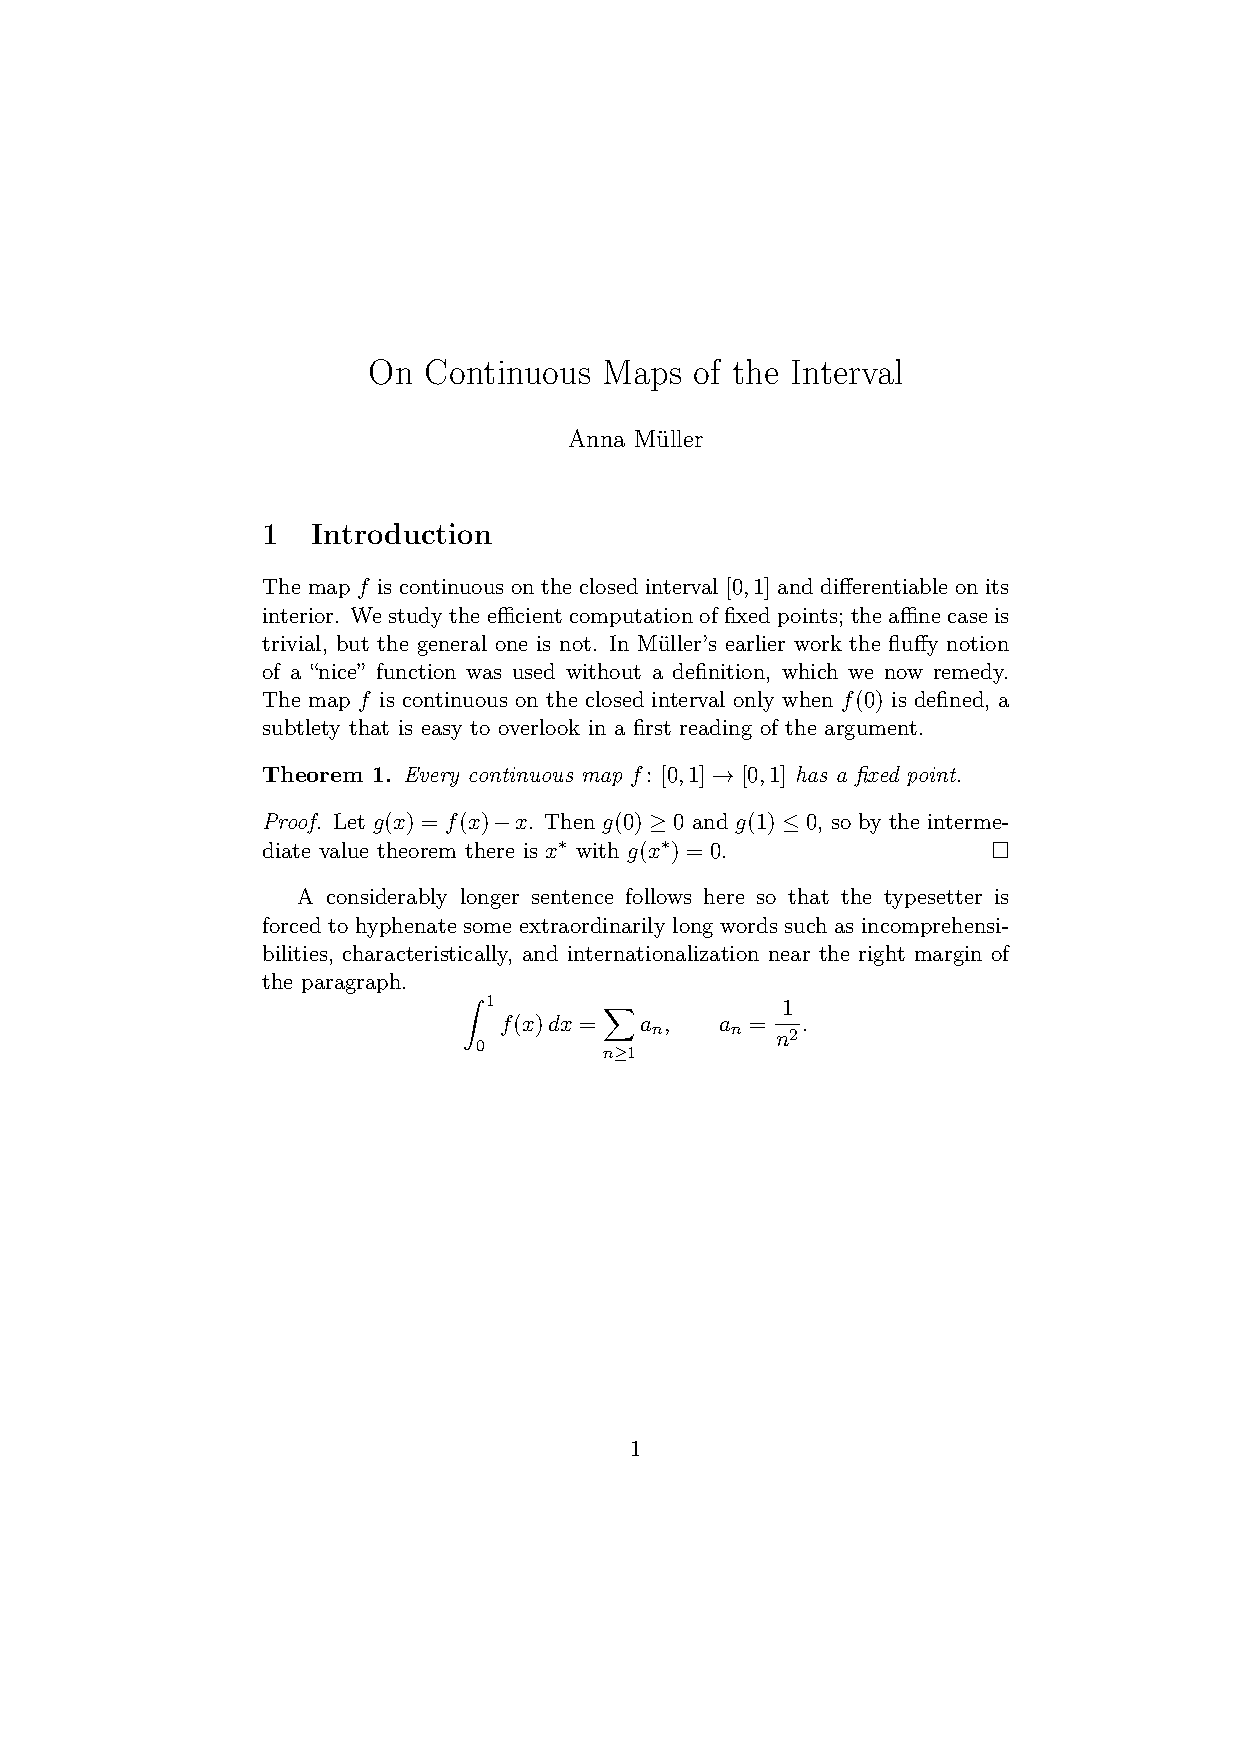
\includegraphics[page=1,width=6cm,trim=80 560 80 120,clip]{../plain/plain.pdf}}
\end{center}

\section{Keller's construction}
Every monotone map on a complete lattice has a least fixed point. Ruffieux's remark
shows that completeness cannot be dropped.

\begin{Form}
\TextField[name=student,value={Anna Mueller},width=5cm]{Name:}
\end{Form}

\begin{thebibliography}{9}
\bibitem{mueller2020} A.~M\"uller. \emph{Ordered sets and their fixed points}. Bachelor thesis, 2020.
\end{thebibliography}
\end{document}
